\documentclass{standalone}
\usepackage{tikz}
\usetikzlibrary{matrix, positioning, shapes, arrows.meta}

\begin{document}

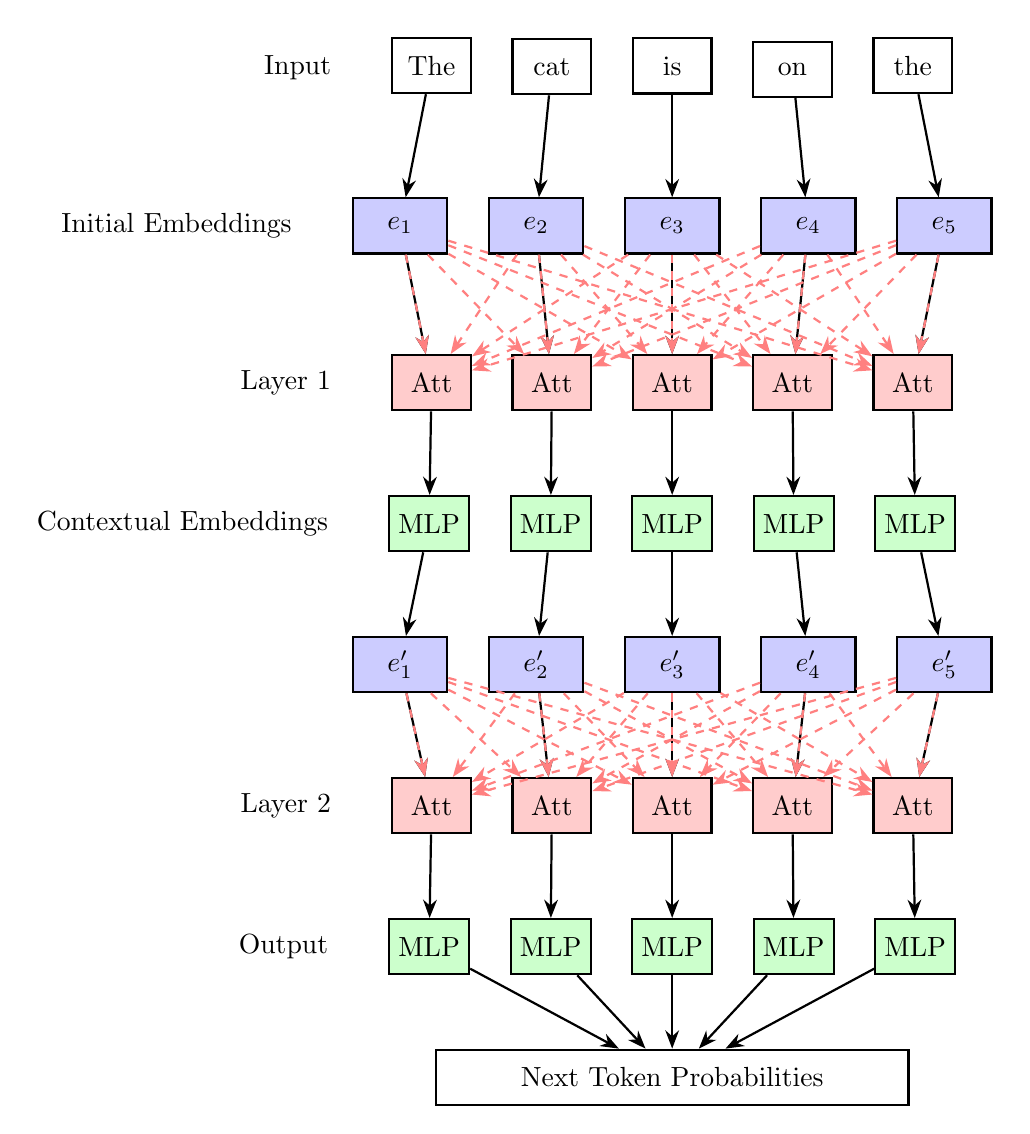
\begin{tikzpicture}[
    word/.style={draw, minimum width=1cm, minimum height=0.7cm},
    embedding/.style={draw, minimum width=1.2cm, minimum height=0.7cm, fill=blue!20},
    attention/.style={draw, minimum width=1cm, minimum height=0.7cm, fill=red!20},
    mlp/.style={draw, minimum width=1cm, minimum height=0.7cm, fill=green!20},
    every path/.style={-Stealth},
    thick
]

% Input words
\matrix (input) [matrix of nodes, nodes=word, column sep=0.5cm] {
    The & cat & is & on & the \\
};

% Initial embeddings
\matrix (embeddings) [below=1cm of input, matrix of nodes, nodes=embedding, column sep=0.5cm] {
    $e_1$ & $e_2$ & $e_3$ & $e_4$ & $e_5$ \\
};

% Layer 1: Self-attention
\matrix (attention1) [below=1cm of embeddings, matrix of nodes, nodes=attention, column sep=0.5cm] {
    Att & Att & Att & Att & Att \\
};

% Layer 1: MLP
\matrix (mlp1) [below=0.8cm of attention1, matrix of nodes, nodes=mlp, column sep=0.5cm] {
    MLP & MLP & MLP & MLP & MLP \\
};

% Contextual Embeddings
\matrix (contextual) [below=0.8cm of mlp1, matrix of nodes, nodes=embedding, column sep=0.5cm] {
    $e_1'$ & $e_2'$ & $e_3'$ & $e_4'$ & $e_5'$ \\
};

% Layer 2: Self-attention
\matrix (attention2) [below=0.8cm of contextual, matrix of nodes, nodes=attention, column sep=0.5cm] {
    Att & Att & Att & Att & Att \\
};

% Layer 2: MLP
\matrix (mlp2) [below=0.8cm of attention2, matrix of nodes, nodes=mlp, column sep=0.5cm] {
    MLP & MLP & MLP & MLP & MLP \\
};

% Output
\node (output) [below=0.8cm of mlp2, draw, minimum width=6cm, minimum height=0.7cm, align=center] {Next Token Probabilities};

% Connections
\foreach \i in {1,2,3,4,5} {
    \draw (input-1-\i) -- (embeddings-1-\i);
    \draw (embeddings-1-\i) -- (attention1-1-\i);
    \draw (attention1-1-\i) -- (mlp1-1-\i);
    \draw (mlp1-1-\i) -- (contextual-1-\i);
    \draw (contextual-1-\i) -- (attention2-1-\i);
    \draw (attention2-1-\i) -- (mlp2-1-\i);
    \draw (mlp2-1-\i) -- (output);
}

% Dashed connections for attention
\foreach \i in {1,2,3,4,5} {
    \foreach \j in {1,2,3,4,5} {
        \draw[dashed, red!50] (embeddings-1-\i) -- (attention1-1-\j);
        \draw[dashed, red!50] (contextual-1-\i) -- (attention2-1-\j);
    }
}

% Labels
\node [left=0.5cm of input] {Input};
\node [left=0.5cm of embeddings] {Initial Embeddings};
\node [left=0.5cm of attention1] {Layer 1};
\node [left=0.5cm of mlp1] {Contextual Embeddings};
\node [left=0.5cm of attention2] {Layer 2};
\node [left=0.5cm of mlp2] {Output};

\end{tikzpicture}

\end{document}